\documentclass{report}

\usepackage{graphicx}
\usepackage{algorithm}
\usepackage{algpseudocode}
\usepackage{float}
\usepackage{adjustbox}
\graphicspath{{graphics/}}


\begin{document}
	\begin{titlepage}
		\centering
		
\includegraphics[scale=0.35]{logo_feup.png}\linebreak
		
		\vspace{1cm}
		
		{\scshape \large Bachelor in Informatics and Computing Engineering
		Information}
		
		\vspace {1cm}
		
		{\scshape\Huge Performance evaluation of a single core \par}
		
		\vfill
		
		{\scshape \large Parallel and Distributed Computing}
		
		\vfill
		
		\Large David \textsc{Preda} - up201904726 \\ Fernando \textsc{Rego} - up201905951 \\ Miguel \textsc{Amorim} - up201907756
		
		\vspace{1cm}
		
		\today
		
	\end{titlepage}

	\tableofcontents
	
	\chapter{Problem Description}
			\paragraph{} The memory system is a hierarchy of storage devices with different capacities, costs, and access times. We can think at this hierarchy as an triangle, where the bottom of the triangle represents the cheaper storage devices with the large amount of memory but the access to memory of this device is extremely slow. On the other hand, the higher top levels of the triangle represents storage devices with small capacities but with an access time much faster then the lower levels storage devices.
			
			\paragraph{} Memory hierarchies work because the memory that tends to be accessed more often is present at the higher levels of the hierarchy causing programs/actions to access more frequently the fastest part of the memory. So the storage at an lower level can be slower, and thus larger and cheaper per bit.
			
			\paragraph{} This project aims to study the effect on the processor performance of the memory hierarchy when accessing large amounts of data. The problem that will be used for this study is the multiplication of two matrices since that this operation with large matrices implies many memory accesses. In parallel, the Performance API (\emph{PAPI}) will be used to collect relevant performance indicators of the program execution.
			
			
	\chapter{Algorithms Explanation}
	
		\paragraph{} In the development of this project, it was used \emph{C++} as the main programming language and three algorithms were developed and optimized to get the best possible results. For the first two algorithms was created a version in the programming language \emph{Rust} to compare the differences, such as duration of execution and memory access, between \emph{Rust} and \emph{C++}.
		
		\section{Matrix Multiplication}
		
			\paragraph{} This is the most basic matrix multiplication' algorithm, which multiplies one line of the first matrix by each column of the second matrix. Directly from the math definition of matrix multiplication $C = A \cdot B$ we obtain:
			
			\begin{center}
				$C_{ij} = \sum_{k=1}^{m} A_{ik} \cdot B_{kj}$
			\end{center}
		
			\paragraph{} From the aforementioned, a simple algorithm can be developed using nested loops over the indices \emph{i}, \emph{j} and \emph{k} to make the necessary operations to obtain the final matrix.
			
			\begin{algorithm}[H]
				\caption{Matrix Multiplication} 
				\begin{algorithmic}[1]
					\State$A\gets $ First Matrix; $B\gets $ Second Matrix;
					\For {$i=0,1,\ldots,size(A)$}
						\For {$j=0,1,\ldots,size(B)$}
							\State $temp\gets $ 0;
							\For {$k=0,1,\ldots,size(A)$}
								\State $temp += A_{ik} \cdot B_{kj}$
							\EndFor
							\State $C_{ij} += temp$
						\EndFor
					\EndFor
					\State\Return $C$;
				\end{algorithmic} 
			\end{algorithm}
		
		\section{Line Matrix Multiplication}
		
			\paragraph{} The line matrix multiplication algorithm is very similar to the first algorithm. The only difference is that, instead of multiply one line of the first matrix by each column of the second matrix, this version multiplies one single element from the first matrix by the correspondent line of the second matrix. 
			
			\paragraph{} To program this algorithm, it is possible to depart from the previous one and change the order of the nested for loops. The following pseudocode makes this more explicit:
			
			\begin{algorithm}[H]
				\caption{Line Matrix Multiplication} 
				\begin{algorithmic}[1]
					\State$A\gets $ First Matrix; $B\gets $ Second Matrix;
					\State$C\gets $ Matrix initialized with 0's;
					\For {$i=0,1,\ldots,size(A)$}
						\For {$k=0,1,\ldots,size(A)$}
							\For {$j=0,1,\ldots,size(B)$}
								\State $C_{ij} += A_{ik} \cdot B_{kj}$
							\EndFor
						\EndFor
					\EndFor
					\State\Return $C$;
				\end{algorithmic} 
			\end{algorithm}
		
		\section{Block Matrix Multiplication}
	
	\chapter{Results and Analysis}
	
		\paragraph{}As requested for this project, the dot product and the line multiplication algorithms were implemented in two languages - C++ and Rust. The block multiplication algorithm was only implemented in C++.
		
		\paragraph{}It is worth noting that the Rust version is using a slightly less efficient implementation than in the C++ one. However, given that the aim of the project is to analyse the effects of memory access on the performance of a single core and not the direct comparison of both languages, the authors believe that this is not a major issue.
	
		\section{Performance Metrics}
		
			\paragraph{}In order to correctly evaluate performance and the correlation between memory access and execution time,  the \emph{Performance Application Programming Interface} (or \emph{PAPI}, for short) was used to collect the number of data cache misses on the L1 and L2 cache level.
			
			\paragraph{}The authors original intention was to measure the percentage of data cache misses relative to the total of data cache accesses. However, due to hardware limitations, \emph{PAPI} wasn't able to register these values. Although this metric could have been of more value to the study, but, sadly, it was not possible to present them.
			
			\paragraph{}Regardless, the execution time for each of the algorithms was also registered, without the use of any external API.
			
		\section{Testing Hardware}
			
		\section{Algorithm Comparison}
		
			\paragraph{}As a way of avoiding any possible misunderstanding, the reader should consider that whenever \emph{cache} is mentioned, the authors mean, specifically, the data cache. Whenever another type of cache, such as the instructions cache, is being mentioned, it should be explicitly clarified.
		
			\subsection{Dot Product vs Line Multiplication}
			
				\paragraph{}Let us start our analysis by comparing the cache misses at both the L1 and L2 levels.
			
				\begin{figure}[H]
					\begin{adjustbox}{center}
						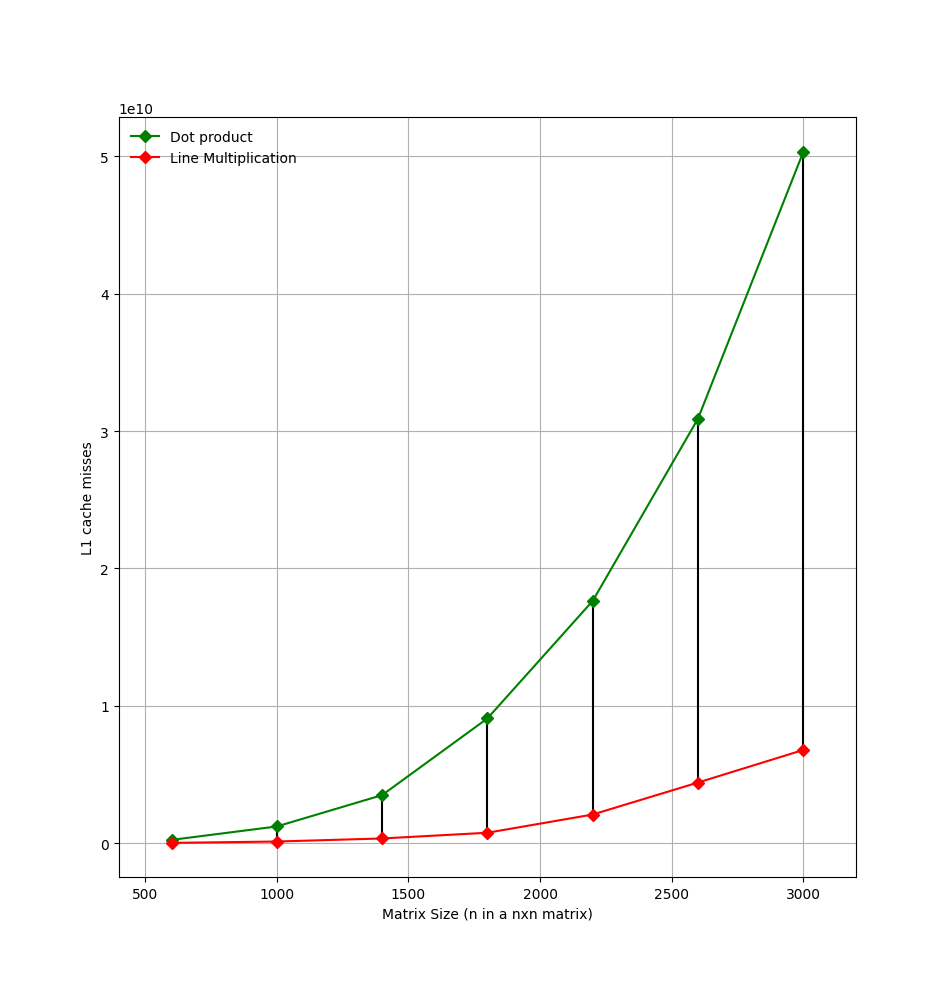
\includegraphics[scale=0.4]{cpp_dot_line_l1.png}
						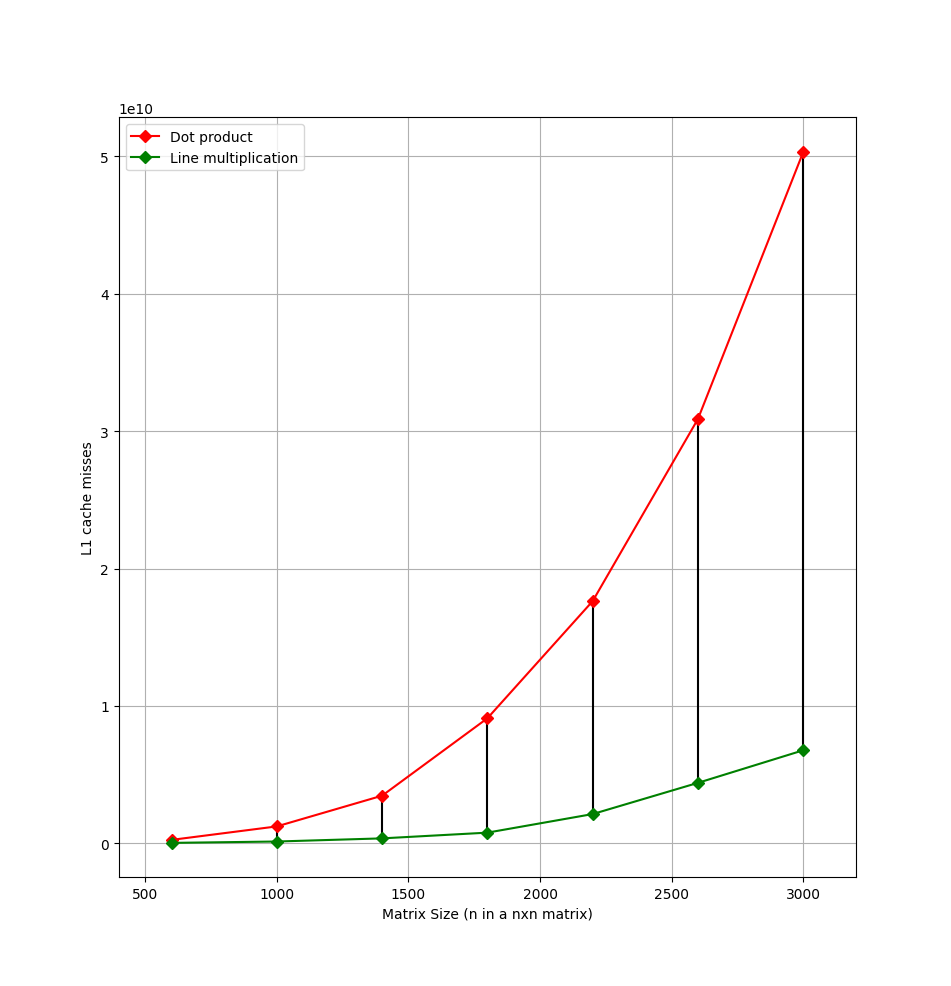
\includegraphics[scale=0.4]{rs_l1_misses.png}
					\end{adjustbox}
					\caption{Comparison of the number of L1 data cache misses of the dot product and line multiplication algorithms for matrices of increasing size. To the left: C++ implementation; to the right: Rust implementation.}
				\end{figure}
			
				\begin{figure}[H]
					\begin{adjustbox}{center}
						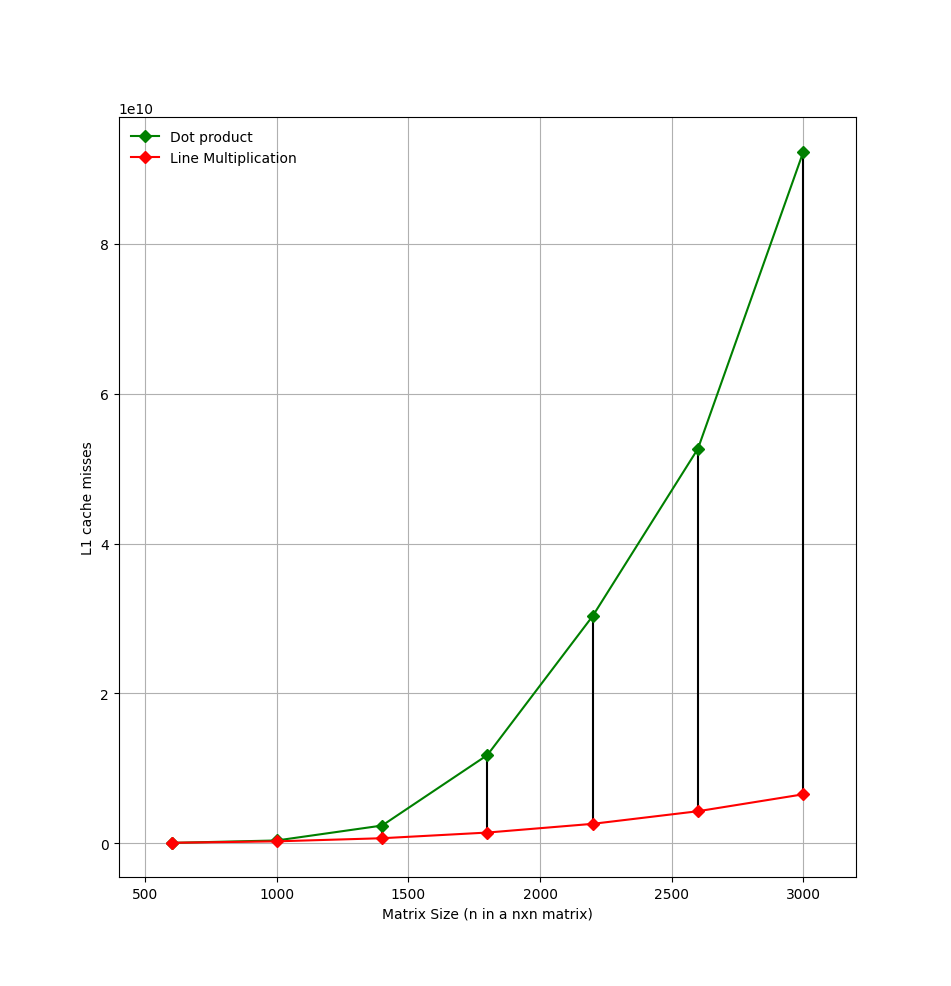
\includegraphics[scale=0.4]{cpp_dot_line_l2.png}
						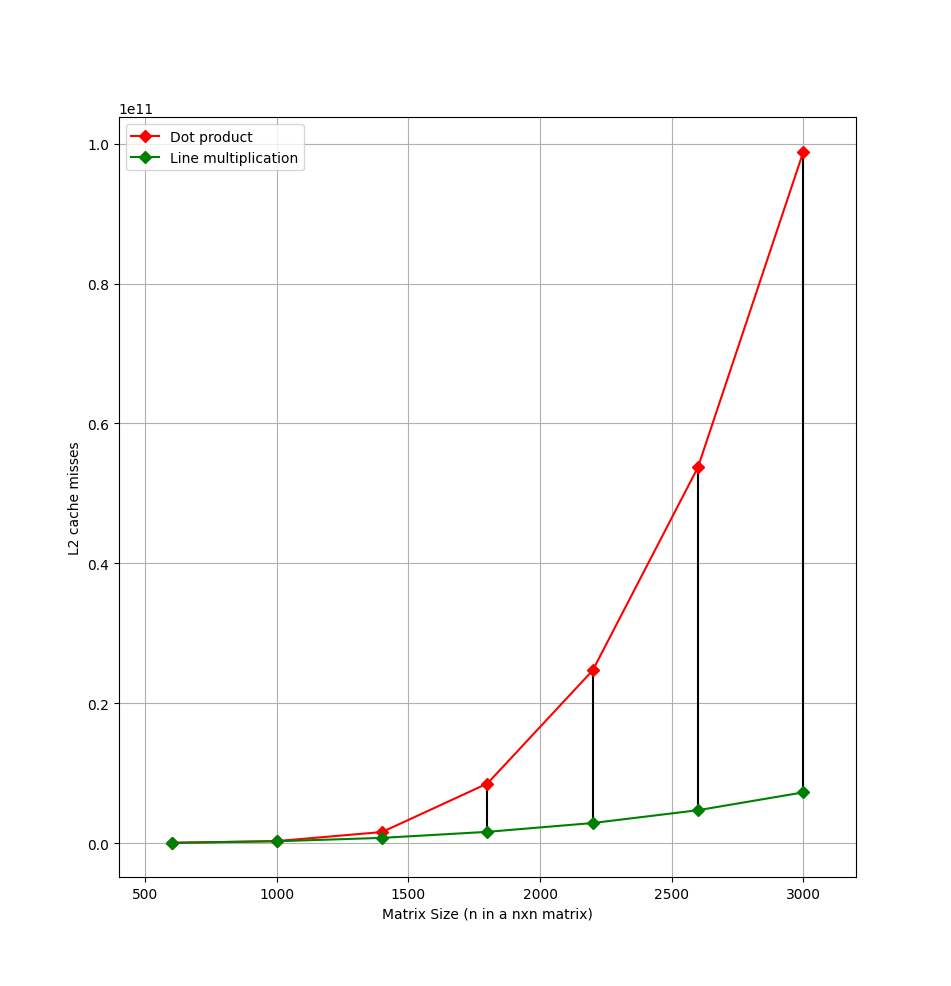
\includegraphics[scale=0.4]{rs_l2_misses.png}
					\end{adjustbox}
					\caption{Comparison of the number of L2 data cache misses of the dot product and line multiplication algorithms for matrices of increasing size. To the left: C++ implementation; to the right: Rust implementation.}
				\end{figure}
			
				\paragraph{}As it is pretty straightforward to see, at both level of caches there is a significant reduction on the number of cache misses from the dot product to the line multiplication algorithm.
				
				\paragraph{}In theory, this should mean a reduced execution time for the line multiplication algorithm, given that it does not have to go through the overhead of higher-level memory access as often as the dot product algorithm.
				
				\paragraph{}Let us now compare the execution time of both algorithms:
			
				\begin{figure}[H]
					\begin{adjustbox}{center}
						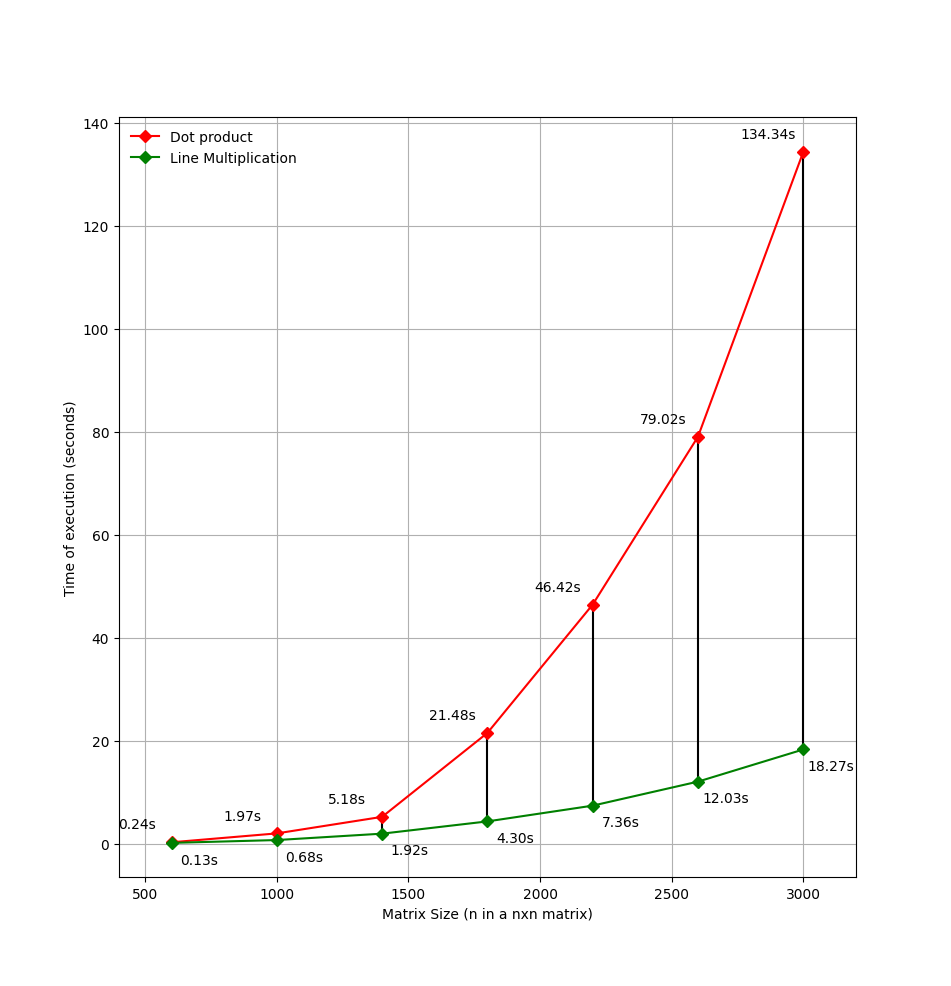
\includegraphics[scale=0.4]{cpp_dot_line_comparison.png}
						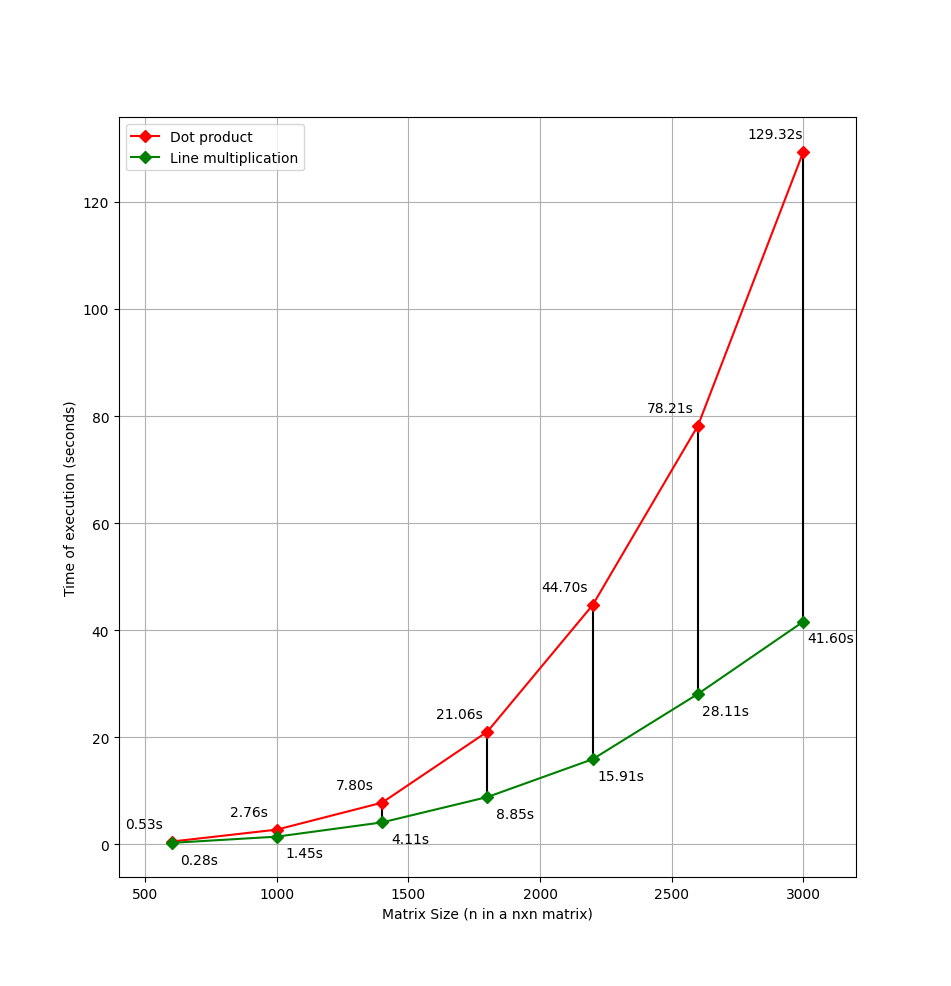
\includegraphics[scale=0.4]{rs_algorithm_comparison.png}
					\end{adjustbox}
					\caption{Comparison of execution time of the dot product and line multiplication algorithms for matrices of increasing size. To the left: C++ implementation; to the right: Rust implementation.}
				\end{figure}
			
				\paragraph{}As expected, the line multiplication algorithm is able to perform all of its operations in a much smaller time, going from 134.34 seconds to only 18.27 seconds for 3000x3000 matrices.
			
			\subsection{Block Multiplication with Different Sizes}
			
				\paragraph{}For the block multiplication algorithm, let us now analyse the metrics inversely - starting with the execution time:
				
				\begin{figure}[H]
					\begin{adjustbox}{center}
						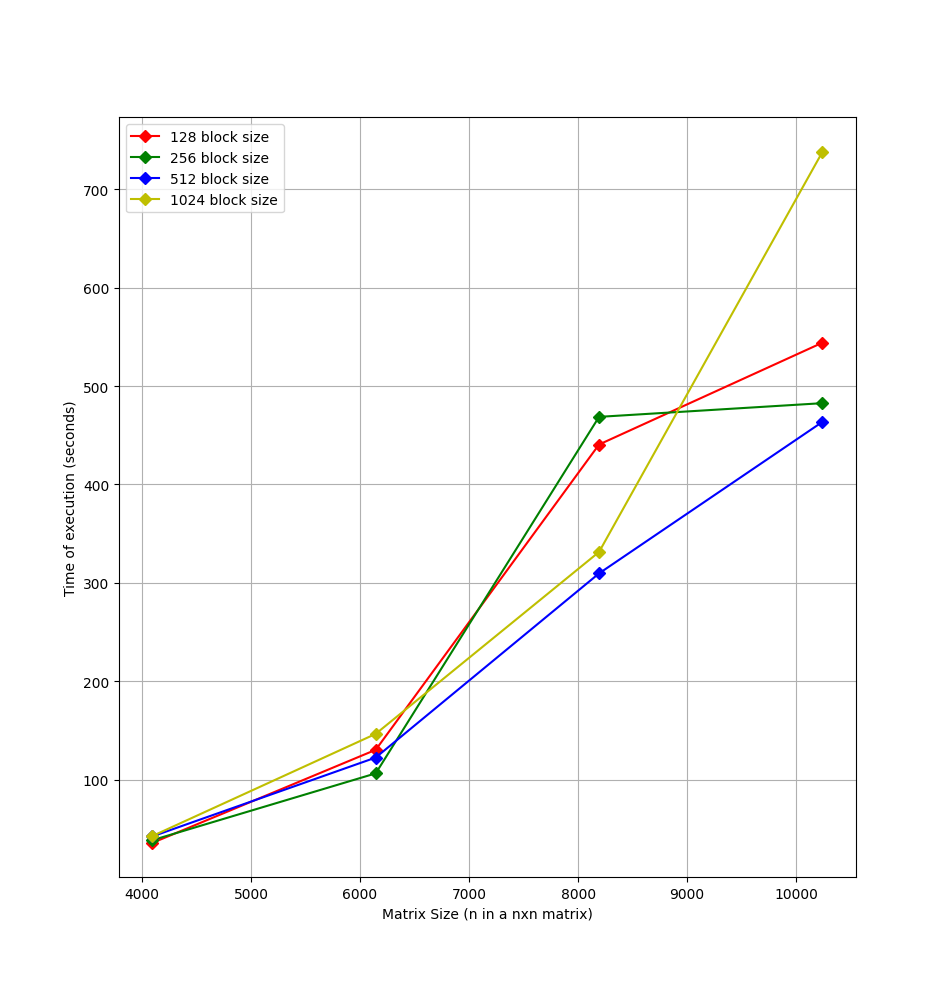
\includegraphics[scale=0.5]{cpp_block_comparison.png}
					\end{adjustbox}
					\caption{Execution time of the block multiplication algorithm for increasing block and matrix sizes.}
				\end{figure}
			
			
				\paragraph{}From the figure, one can conclude that, on average, the 512 block size version of the algorithm performs better than the others.
				
				\paragraph{}With this in mind, let us now analyse the cache misses per millisecond:
				
				\begin{figure}[H]
					\begin{adjustbox}{center}
						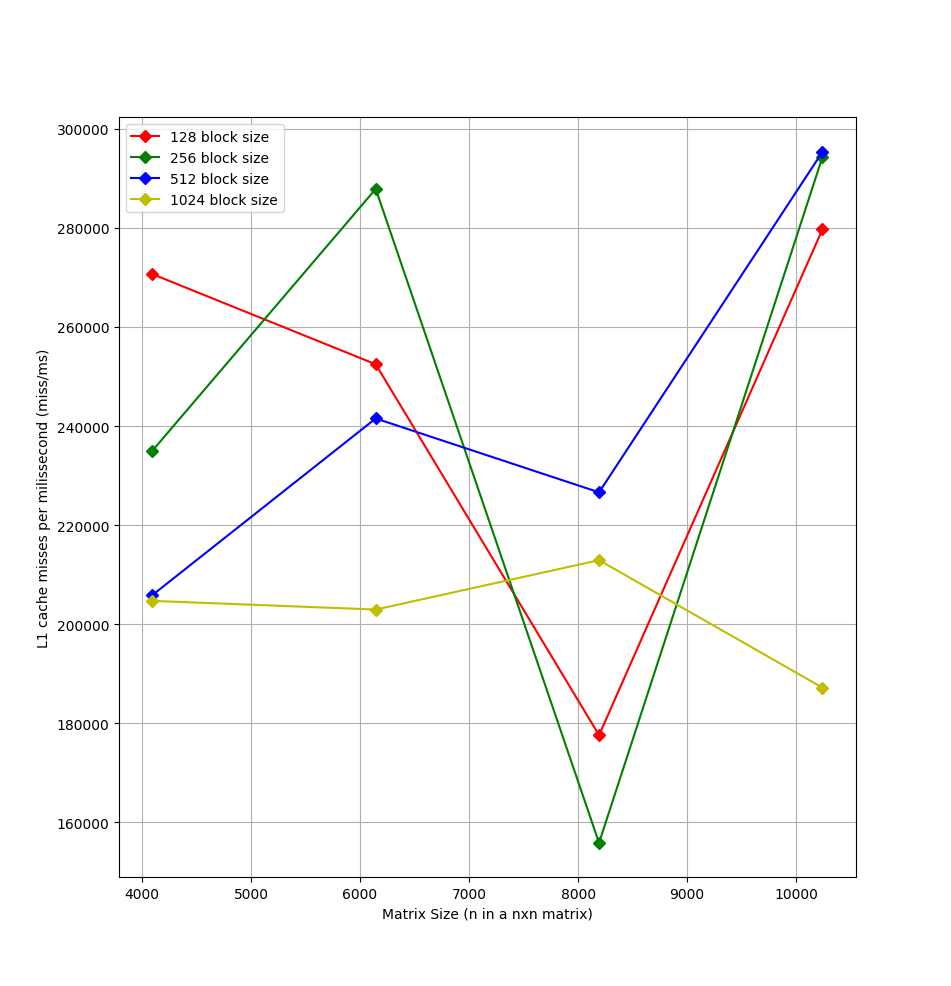
\includegraphics[scale=0.4]{cpp_block_l1_misses.png}
						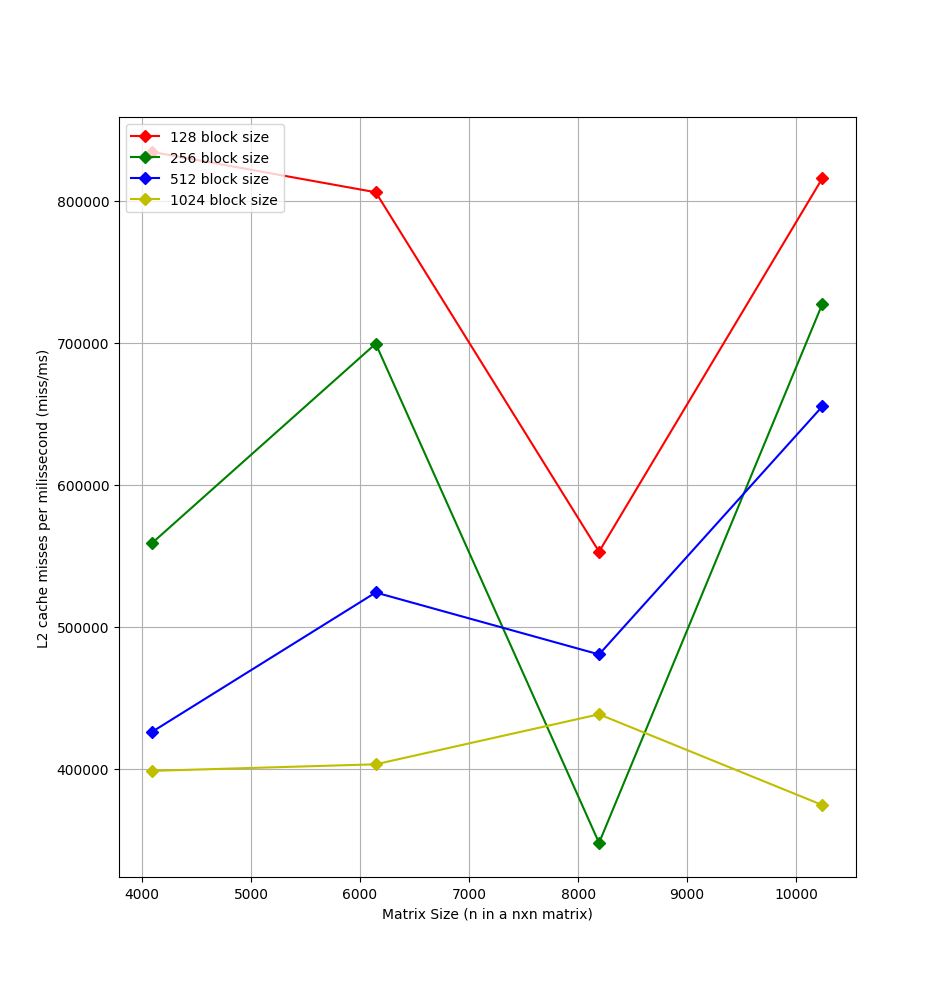
\includegraphics[scale=0.4]{cpp_block_l2_misses.png}
					\end{adjustbox}
					\caption{Comparison of data cache misses of the block multiplication for increasing block and matrix sizes. To the left: L1 cache misses per millisecond; to the right: L2 cache misses per millisecond.}
				\end{figure}
			
				\paragraph{}Contrary to the expected, the 512 block size version does not have a lower cache miss per millisecond rate. Therefore, it is not possible to relate the better performance with the accesses to memory.
				
				\paragraph{}However, after some research, the authors concluded that the better performance could be related to computational intensity. Bundling together arithmetic operations can lead to faster performance, depending on the cache size of the underlying hardware and the load of the operations. \cite{1}
		
			\subsection{Line Multiplication vs Block Multiplication}
				
				\paragraph{}Finally, let us compare the line multiplication algorithm with block multiplication algorithm. As it performed better, the 512 block size version will be the one used to represent the block approach.
				
				\paragraph{}As in the first comparison, let's first verify how both algorithms behave cache-wise:
				
				\begin{figure}[H]
					\begin{adjustbox}{center}
						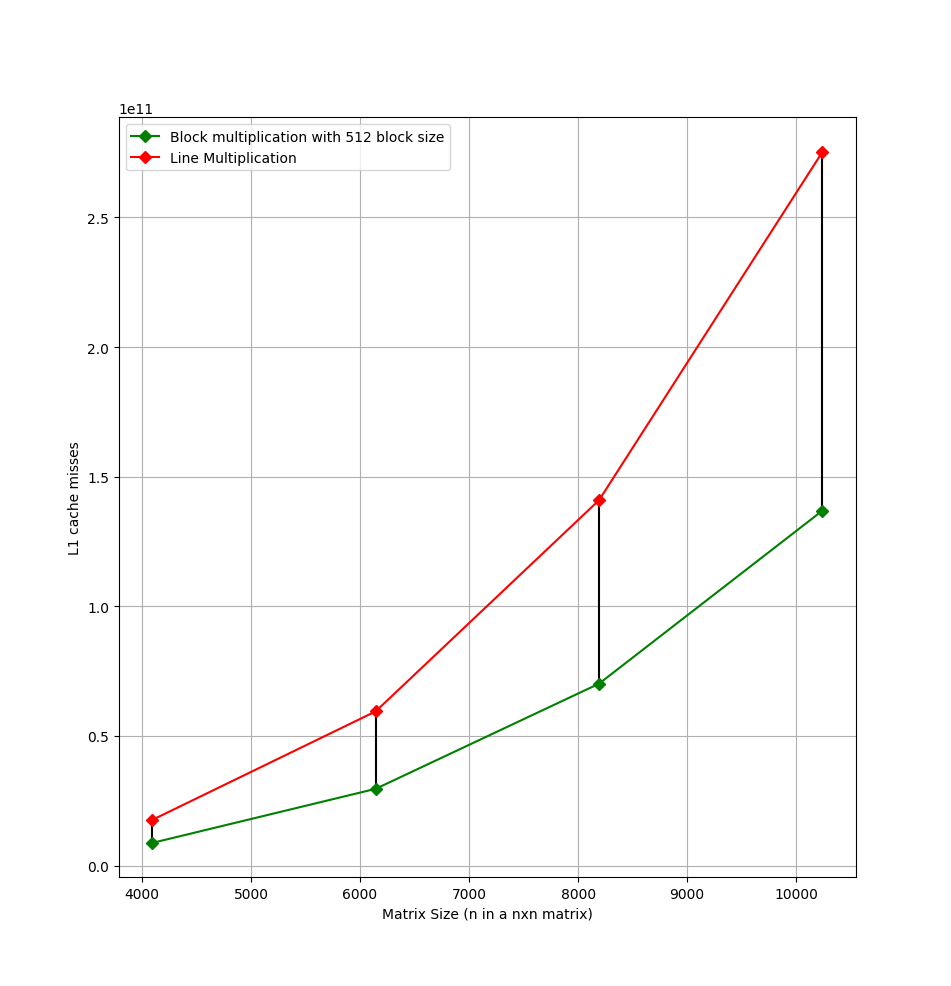
\includegraphics[scale=0.4]{cpp_line_block_l1.png}
						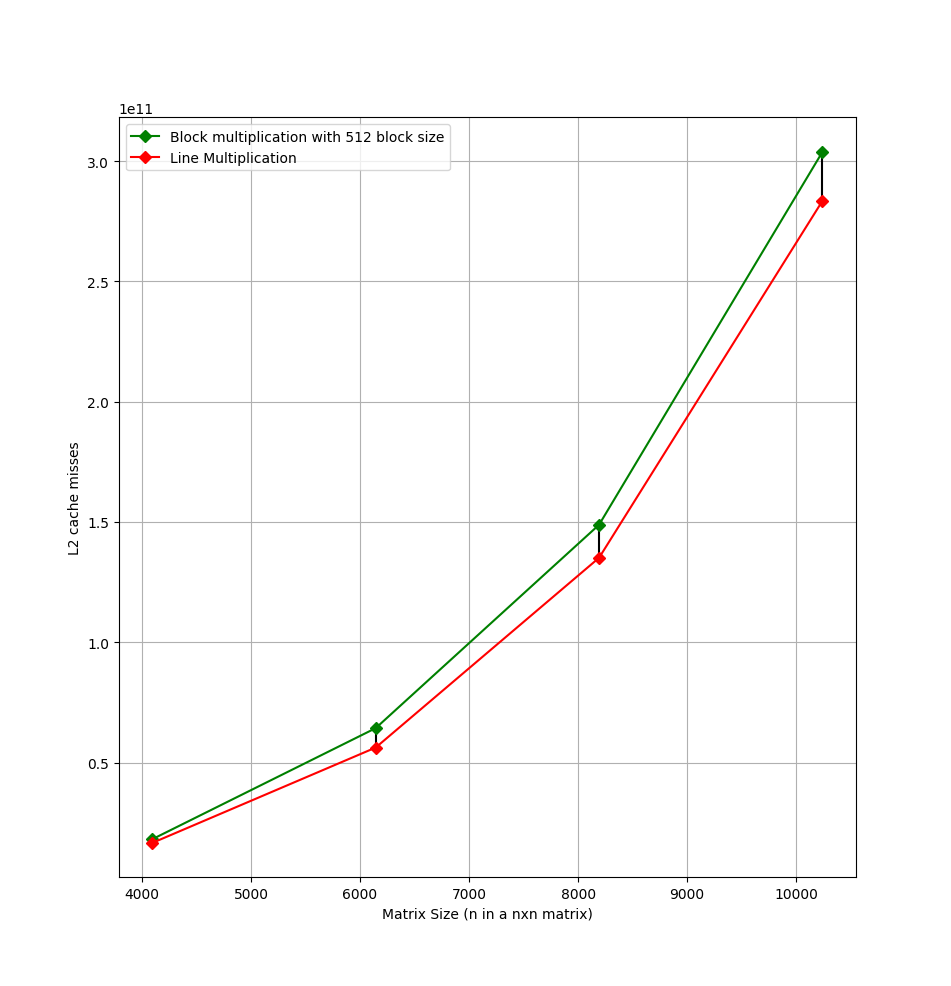
\includegraphics[scale=0.4]{cpp_line_block_l2.png}
					\end{adjustbox}
					\caption{Comparison of data cache misses between the line multiplication algorithm and the block multiplication algorithm for increasing matrices. To the left: Total L1 data cache misses; to the right: Total L2 data cache misses.}
				\end{figure}
			
				\paragraph{}The total L1 data cache misses are drastically smaller for the block multiplication algorithm. However, they are almost on par at the L2 cache level, with the line multiplication having less misses.
				
				\paragraph{}Let us now see how if there is any correlation with the execution time:
				
				\begin{figure}[H]
					\begin{adjustbox}{center}
						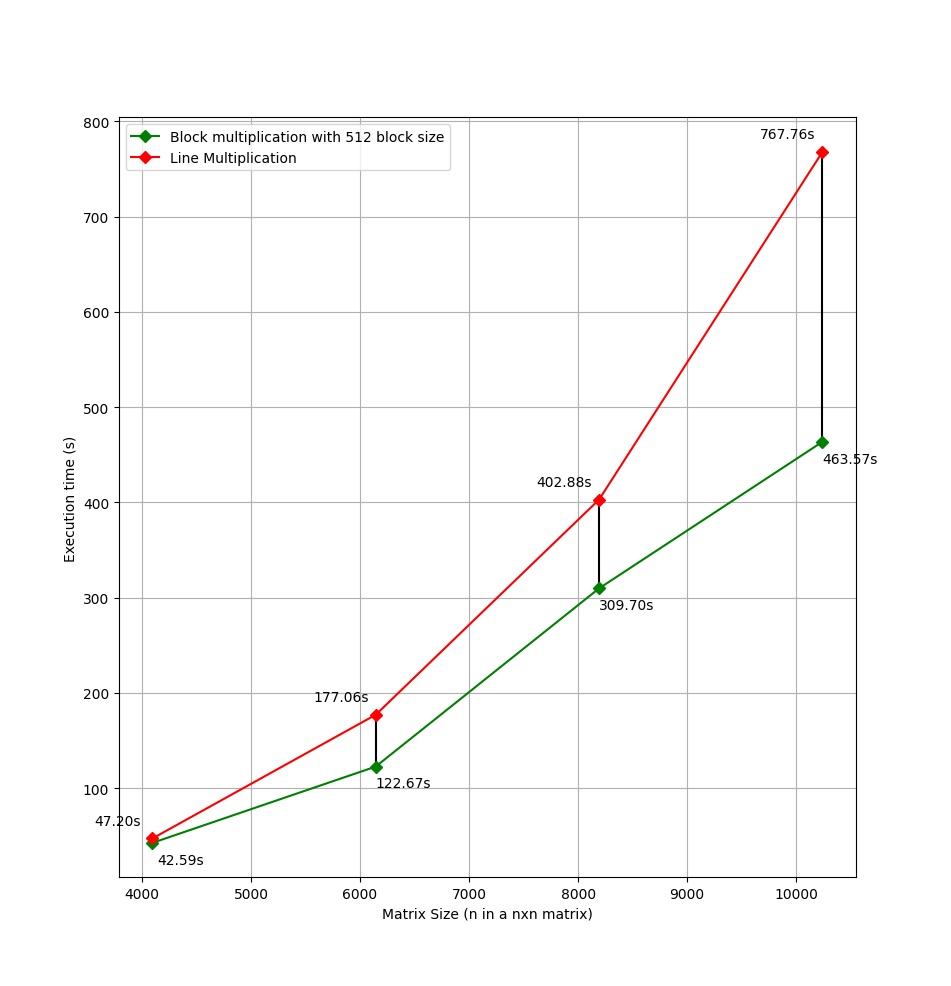
\includegraphics[scale=0.4]{cpp_line_block_comparison.png}
					\end{adjustbox}
					\caption{Comparison of execution time between the line multiplication algorithm and block multiplication algorithm for increasing matrices.}
				\end{figure}
			
				\paragraph{}The block multiplication algorithm, as the matrices increase in size, starts to take less and less time, when comparing it with the line multiplication algorithm. This difference is analogous to what is seen on the graph comparing the L1 data cache misses between the two algorithms.
				
				\paragraph{}We, therefore, conclude that the block approach leads to a better performance due to being less heavy on higher-level memory access.
			
		\section{Language Comparison}
		
		\paragraph{}Finally, a comparison between both languages is now due. The line multiplication algorithm will be used as the basis for this comparison, as it is the best performing one that is implemented in both language. 
		
		\paragraph{}Let us start by comparing data cache misses: 
	
	\chapter{Conclusions}
	
	\addcontentsline{toc}{chapter}{Bibliography}
	\begin{thebibliography}{1}
		\bibitem{1}
		JAYAWEERA, Malith \textit{Blocked Matrix Multiplication}
		\\\texttt{https://malithjayaweera.com/2020/07/blocked-matrix-multiplication/}
	\end{thebibliography}
	
\end{document}